\documentclass[10pt,final,a4paper,oneside,onecolumn]{article}

%%==========================================================================
%% Packages
%%==========================================================================
\usepackage[a4paper,left=3.5cm,right=3.5cm,top=3cm,bottom=3cm]{geometry} %% change page layout; remove for IEEE paper format
\usepackage[T1]{fontenc}                        %% output font encoding for international characters (e.g., accented)
\usepackage[cmex10]{amsmath}                    %% math typesetting; consider using the [cmex10] option
\usepackage{amssymb}                            %% special (symbol) fonts for math typesetting
\usepackage{amsthm}                             %% theorem styles
\usepackage{dsfont}                             %% double stroke roman fonts: the real numbers R: $\mathds{R}$
\usepackage{mathrsfs}                           %% formal script fonts: the Laplace transform L: $\mathscr{L}$
\usepackage[pdftex]{graphicx}                   %% graphics control; use dvips for TeXify; use pdftex for PDFTeXify
\usepackage{array}                              %% array functionality (array, tabular)
\usepackage{upgreek}                            %% upright Greek letters; add the prefix 'up', e.g. \upphi
\usepackage{stfloats}                           %% improved handling of floats
\usepackage{multirow}                           %% cells spanning multiple rows in tables
%\usepackage{subfigure}                         %% subfigures and corresponding captions (for use with IEEEconf.cls)
\usepackage{fancyhdr}                           %% page headers and footers
\usepackage[official,left]{eurosym}             %% the euro symbol; command: \euro
\usepackage{appendix}                           %% appendix layout
\usepackage{xspace}                             %% add space after macro depending on context
\usepackage{verbatim}                           %% provides the comment environment
\usepackage[dutch,USenglish]{babel}             %% language support
\usepackage{wrapfig}                            %% wrapping text around figures
\usepackage{longtable}                          %% tables spanning multiple pages
\usepackage{pgfplots}                           %% support for TikZ figures (Matlab/Python)
\pgfplotsset{compat=1.14}						%% Run in backwards compatibility mode
\usepackage[breaklinks=true,hidelinks,          %% implement hyperlinks (dvips yields minor problems with breaklinks;
bookmarksnumbered=true]{hyperref}   %% IEEEtran: set bookmarks=false)
%\usepackage[hyphenbreaks]{breakurl}            %% allow line breaks in URLs (don't use with PDFTeX)
\usepackage[final]{pdfpages}                    %% Include other pdfs
\usepackage[capitalize]{cleveref}				%% Referensing to figures, equations, etc.
\usepackage{units}								%% Appropriate behavior of units
\usepackage[utf8]{inputenc}   				 	%% utf8 support (required for biblatex)
\usepackage{csquotes}							%% Quoted texts are typeset according to rules of main language
\usepackage[style=ieee,doi=false,isbn=false,url=false,date=year,minbibnames=15,maxbibnames=15,backend=biber]{biblatex}
%\renewcommand*{\bibfont}{\footnotesize}		%% Use this for papers
\setlength{\biblabelsep}{\labelsep}
\bibliography{../../bib}
\usepackage{subcaption}

%%==========================================================================
%% Define reference stuff
%%==========================================================================
\crefname{figure}{Figure}{Figures}
\crefname{equation}{}{}

%%==========================================================================
%% Define header/title stuff
%%==========================================================================
\newcommand{\progressreportnumber}{22}
\renewcommand{\author}{Erwin de Gelder}
\renewcommand{\date}{September 11, 2019}
\renewcommand{\title}{Performance assessment of automated vehicles using real-world driving scenarios}

%%==========================================================================
%% Fancy headers and footers
%%==========================================================================
\pagestyle{fancy}                                       %% set page style
\fancyhf{}                                              %% clear all header & footer fields
\fancyhead[L]{Progress report \progressreportnumber}    %% define headers (LE: left field/even pages, etc.)
\fancyhead[R]{\author, \date}                           %% similar
\fancyfoot[C]{\thepage}                                 %% define footer

\newlength{\figurewidth}
\begin{document}
	
\begin{center}
	\begin{tabular}{c}
		\title \\ \\
		\textbf{\huge Progress report \progressreportnumber} \\ \\
		\author \\ 
		\date
	\end{tabular}
\end{center}

\section{Previous meeting minutes}

\begin{itemize}
	\item I suggested to follow the course \emph{Writing a dissertation}, because in this course, I would write the introduction of the PhD dissertation. Bart suggested, however, that it would be better to look for another course, because writing the introduction of the dissertation should not be too difficult. 
	\item We discussed the planning for my PhD. According to the proposed planning, I would work on four different topics. It has been suggested that I should work at most on three topics at the same time. Furthermore, Bart mentioned that writing the dissertation takes around two weeks per chapter, assuming that each chapter is based on an already published paper, whereas I thought writing the dissertation would take a year.
	\item We shortly discussed the work on the \emph{scenario risk} paper. The proposed method was based on ISO~26262 \cite{ISO26262}. Bart suggested that it would be better to write the proposed method from a more general perspective, because standards, such as ISO~26262, are not necessarily the best scientific source. In a subsection, we can still explain the relation between the proposed method and ISO~26262.
\end{itemize}

\section{Summary of work}

\begin{itemize}
	\item I submitted the ontology paper. The paper is now under review.
	
	\item I worked on the \emph{scenario risk estimation}:
	\begin{itemize}
		\item I did a literature search on quantifying the risk. It turned out that this is harder than I thought. There are many ``risk estimation'' techniques, e.g., Failure Mode and Effect Analysis (FMEA), Structured What If Technique (SWIFT), Hazard and Operability (HAZOP), and Systems-Theoretic Processes Analysis (STPA). It seems, however, that these methods focus on identifying the different hazards. I could not find a method for quantification of a risk of a hazard.
		
		For example, in \cite{tokody2017overview}, an FMEA is performed for ``intelligent vehicles''. The risk of each failure is simply calculated by multiplying the \emph{failure extent}, the \emph{frequency}, and the \emph{recognisability}. In \cite{tokody2017overview}, there is no information on how these numbers are estimated. On the one hand, this shows that our paper is original and no similar work (that is known to me) is done before. On the other hand, it might be good if there is already some work that can be used as a reference.
		
		\item I want to include a case study. In my previous papers, I always considered the ``obvious'' scenario categories \emph{lead vehicle braking} \cite{deGelder2017assessment, degelder2019completeness} or \emph{cut-in} \cite{degelder2019risk}. For this paper, I want to work out more scenario categories to give the case study more significance. In \cref{fig:scenarios}, the scenario categories that I want to consider for the case study are shown. To simplify the case study, I want to only consider highway driving.
		
		\item The data I want to use for the analysis consists of 60 hours of driving, of which roughly 50\% on highway \cite{paardekooper2019dataset6000km}. The scenarios need to be identified in the data. I want to do this automatically. I did some Python programming for this, but it is not yet finished. 
	\end{itemize}

	\item In CETRAN, we finished a first version of a report describing the overall methodology for assessing an autonomous vehicle. This version is reviewed by the Land Transport Authority. Based on their feedback, we will improve the report.
\end{itemize}

\setlength{\figurewidth}{0.49\textwidth}
\begin{figure}
	\begin{subfigure}{0.49\textwidth}
		\input{scenarios/"lead braking".tikz}
		\vspace{-1em}
		\caption{Lead vehicle braking.}
		\vspace{1em}
	\end{subfigure}
	\begin{subfigure}{0.49\textwidth}
		\input{scenarios/"lead braking overtaking".tikz}
		\vspace{-1em}
		\caption{Lead vehicle braking with overtaking vehicle.}
		\vspace{1em}
	\end{subfigure}
	\begin{subfigure}{0.49\textwidth}
		\input{scenarios/"slow lead".tikz}
		\vspace{-1em}
		\caption{Slow lead vehicle.}
		\vspace{1em}
	\end{subfigure}
	\begin{subfigure}{0.49\textwidth}
		\input{scenarios/"slow lead overtaking".tikz}
		\vspace{-1em}
		\caption{Slow lead vehicle with overtaking vehicle.}
		\vspace{1em}
	\end{subfigure}
	\begin{subfigure}{0.49\textwidth}
		% This file was created by matplotlib2tikz v0.6.17.
\begin{tikzpicture}

\definecolor{color0}{rgb}{0.8,1,0.8}
\definecolor{color1}{rgb}{0,0.4375,0.75}

\begin{axis}[
xmin=-15, xmax=15,
ymin=-5, ymax=5,
width=\figurewidth,
height=0.33\figurewidth,
tick align=outside,
xticklabel style = {align=center,text width=1},
yticklabel style = {align=right,text width=1},
tick pos=left,
x grid style={white!69.01960784313725!black},
y grid style={white!69.01960784313725!black},
axis background/.style={fill=color0},
ticks=none,
scale only axis
]
\path [draw=white!80.0!black, fill=white!80.0!black] (axis cs:-15.0004761151639,2.79999995952042)
--(axis cs:0.0851092925312272,2.80256512954621)
--(axis cs:4.95111961061006,2.79829127699914)
--(axis cs:5.14664116816982,-1.39487383099742)
--(axis cs:0.0860615228589551,-2.79743478949463)
--(axis cs:-14.9995238848361,-2.79999995952042)
--cycle;

\path [draw=white, fill=white] (axis cs:-13.7375163208298,-1.54978534825389)
--(axis cs:-13.7375673331688,-1.24978535259098)
--(axis cs:-12.107552053032,-1.33950818424803)
--(axis cs:-12.052562256295,-1.27949883285331)
--(axis cs:-12.0150775605388,-1.18949245761206)
--(axis cs:-12.0150877630066,-1.12949245847948)
--(axis cs:-12.3550877580912,-1.12955027246366)
--(axis cs:-11.882643878495,-0.79946993280057)
--(axis cs:-11.2375877742469,-1.12936025150094)
--(axis cs:-11.7875877662956,-1.12945377412242)
--(axis cs:-11.78756736136,-1.24945377238758)
--(axis cs:-11.8250520571161,-1.33946014762882)
--(axis cs:-11.9200316508071,-1.45947629980133)
--cycle;

\path [draw=white, fill=white] (axis cs:-8.71307612613488,-1.54893098675345)
--(axis cs:-8.71312713847387,-1.24893099109055)
--(axis cs:-7.08311185833707,-1.3386538227476)
--(axis cs:-7.0281220616,-1.27864447135287)
--(axis cs:-6.99063736584383,-1.18863809611163)
--(axis cs:-6.99064756831163,-1.12863809697905)
--(axis cs:-7.33064756339625,-1.12869591096323)
--(axis cs:-6.85820368380007,-0.798615571300139)
--(axis cs:-6.21314757955194,-1.12850589000051)
--(axis cs:-6.7631475716006,-1.12859941262199)
--(axis cs:-6.763127166665,-1.24859941088715)
--(axis cs:-6.80061186242117,-1.33860578612839)
--(axis cs:-6.89559145611216,-1.4586219383009)
--cycle;

\path [draw=white, fill=white] (axis cs:-3.68863593143991,-1.54807662525302)
--(axis cs:-3.6886869437789,-1.24807662959012)
--(axis cs:-2.0586716636421,-1.33779946124717)
--(axis cs:-2.00368186690503,-1.27779010985244)
--(axis cs:-1.96619717114886,-1.1877837346112)
--(axis cs:-1.96620737361666,-1.12778373547862)
--(axis cs:-2.30620736870128,-1.1278415494628)
--(axis cs:-1.8337634891051,-0.797761209799709)
--(axis cs:-1.18870738485697,-1.12765152850008)
--(axis cs:-1.73870737690563,-1.12774505112156)
--(axis cs:-1.73868697197003,-1.24774504938672)
--(axis cs:-1.7761716677262,-1.33775142462796)
--(axis cs:-1.87115126141719,-1.45776757680047)
--cycle;

\path [draw=white, fill=white] (axis cs:1.33580426325506,-1.54722226375259)
--(axis cs:1.33575325091607,-1.24722226808969)
--(axis cs:2.96576853105287,-1.33694509974674)
--(axis cs:3.02075832778994,-1.27693574835201)
--(axis cs:3.05824302354611,-1.18692937311077)
--(axis cs:3.05823282107831,-1.12692937397819)
--(axis cs:2.71823282599369,-1.12698718796237)
--(axis cs:3.19067670558987,-0.796906848299278)
--(axis cs:3.835732809838,-1.12679716699965)
--(axis cs:3.28573281778934,-1.12689068962112)
--(axis cs:3.28575322272494,-1.24689068788629)
--(axis cs:3.24826852696877,-1.33689706312753)
--(axis cs:3.15328893327778,-1.45691321530004)
--cycle;

\path [draw=white!80.0!black, fill=white!80.0!black] (axis cs:4.95111961061006,2.79829127699914)
--(axis cs:10,2.8)
--(axis cs:15,2.8)
--(axis cs:15,0)
--(axis cs:10,0)
--(axis cs:5.14664116816982,-1.39487383099742)
--cycle;

\addplot [semithick, black, forget plot]
table {%
-15.0004761151639 2.79999995952042
0.0851092925312272 2.80256512954621
4.95111961061006 2.79829127699914
};
\addplot [semithick, black, forget plot]
table {%
5.14664116816982 -1.39487383099742
0.0860615228589551 -2.79743478949463
-14.9995238848361 -2.79999995952042
};
\addplot [semithick, black, forget plot]
table {%
-15 0
-14.5214818862195 8.13677619457745e-05
};
\addplot [semithick, black, forget plot]
table {%
-12.6074094310976 0.000406838809728873
-11.6503732035367 0.000569574333620422
};
\addplot [semithick, black, forget plot]
table {%
-9.73630074841479 0.00089504538140352
-8.77926452085385 0.00105778090529507
};
\addplot [semithick, black, forget plot]
table {%
-6.86519206573195 0.00138325195307817
-5.90815583817101 0.00154598747696972
};
\addplot [semithick, black, forget plot]
table {%
-3.99408338304911 0.00187145852475281
-3.03704715548817 0.00203419404864436
};
\addplot [semithick, black, forget plot]
table {%
-1.12297470036627 0.00235966509642746
-0.165938472805329 0.00252240062031901
};
\addplot [semithick, black, forget plot]
table {%
1.74813398231657 0.00284787166810215
2.70517020987751 0.00301060719199373
};
\addplot [semithick, black, forget plot]
table {%
4.6192426649994 0.00333607823977688
5.09776077877988 0.00341744600172267
};
\addplot [semithick, white, forget plot]
table {%
-13.7375163208298 -1.54978534825389
-13.7375673331688 -1.24978535259098
-12.107552053032 -1.33950818424803
-12.052562256295 -1.27949883285331
-12.0150775605388 -1.18949245761206
-12.0150877630066 -1.12949245847948
-12.3550877580912 -1.12955027246366
-11.882643878495 -0.79946993280057
-11.2375877742469 -1.12936025150094
-11.7875877662956 -1.12945377412242
-11.78756736136 -1.24945377238758
-11.8250520571161 -1.33946014762882
-11.9200316508071 -1.45947629980133
-13.7375163208298 -1.54978534825389
};
\addplot [semithick, white, forget plot]
table {%
-8.71307612613488 -1.54893098675345
-8.71312713847387 -1.24893099109055
-7.08311185833707 -1.3386538227476
-7.0281220616 -1.27864447135287
-6.99063736584383 -1.18863809611163
-6.99064756831163 -1.12863809697905
-7.33064756339625 -1.12869591096323
-6.85820368380007 -0.798615571300139
-6.21314757955194 -1.12850589000051
-6.7631475716006 -1.12859941262199
-6.763127166665 -1.24859941088715
-6.80061186242117 -1.33860578612839
-6.89559145611216 -1.4586219383009
-8.71307612613488 -1.54893098675345
};
\addplot [semithick, white, forget plot]
table {%
-3.68863593143991 -1.54807662525302
-3.6886869437789 -1.24807662959012
-2.0586716636421 -1.33779946124717
-2.00368186690503 -1.27779010985244
-1.96619717114886 -1.1877837346112
-1.96620737361666 -1.12778373547862
-2.30620736870128 -1.1278415494628
-1.8337634891051 -0.797761209799709
-1.18870738485697 -1.12765152850008
-1.73870737690563 -1.12774505112156
-1.73868697197003 -1.24774504938672
-1.7761716677262 -1.33775142462796
-1.87115126141719 -1.45776757680047
-3.68863593143991 -1.54807662525302
};
\addplot [semithick, white, forget plot]
table {%
1.33580426325506 -1.54722226375259
1.33575325091607 -1.24722226808969
2.96576853105287 -1.33694509974674
3.02075832778994 -1.27693574835201
3.05824302354611 -1.18692937311077
3.05823282107831 -1.12692937397819
2.71823282599369 -1.12698718796237
3.19067670558987 -0.796906848299278
3.835732809838 -1.12679716699965
3.28573281778934 -1.12689068962112
3.28575322272494 -1.24689068788629
3.24826852696877 -1.33689706312753
3.15328893327778 -1.45691321530004
1.33580426325506 -1.54722226375259
};
\addplot [semithick, black, forget plot]
table {%
4.95111961061006 2.79829127699914
10 2.8
15 2.8
};
\addplot [semithick, black, forget plot]
table {%
15 0
10 0
5.14664116816982 -1.39487383099742
};
\path [draw=black, fill=color1] (axis cs:-12.25,1.40401785714286)
--(axis cs:-12.2418918918919,1.92633928571429)
--(axis cs:-12.1851351351351,2.12723214285714)
--(axis cs:-12.1040540540541,2.19955357142857)
--(axis cs:-11.9743243243243,2.24776785714286)
--(axis cs:-11.5121621621622,2.30401785714286)
--(axis cs:-8.09864864864865,2.26383928571429)
--(axis cs:-8.00945945945946,2.20758928571429)
--(axis cs:-7.87162162162162,2.03080357142857)
--(axis cs:-7.81486486486487,1.83794642857143)
--(axis cs:-7.75,1.40401785714286)
--(axis cs:-7.75,1.39598214285714)
--(axis cs:-7.81486486486487,0.962053571428571)
--(axis cs:-7.87162162162162,0.769196428571429)
--(axis cs:-8.00945945945946,0.592410714285714)
--(axis cs:-8.09864864864865,0.536160714285714)
--(axis cs:-11.5121621621622,0.495982142857143)
--(axis cs:-11.9743243243243,0.552232142857143)
--(axis cs:-12.1040540540541,0.600446428571428)
--(axis cs:-12.1851351351351,0.672767857142857)
--(axis cs:-12.2418918918919,0.873660714285714)
--(axis cs:-12.25,1.39598214285714)
--cycle;

\path [draw=black, fill=color1] (axis cs:-9.33108108108108,2.23169642857143)
--(axis cs:-9.33918918918919,2.43258928571429)
--(axis cs:-9.33108108108108,2.48080357142857)
--(axis cs:-9.29864864864865,2.45669642857143)
--(axis cs:-9.25,2.24776785714286)
--cycle;

\path [draw=black, fill=color1] (axis cs:-9.33108108108108,0.568303571428571)
--(axis cs:-9.33918918918919,0.367410714285714)
--(axis cs:-9.33108108108108,0.319196428571428)
--(axis cs:-9.29864864864865,0.343303571428571)
--(axis cs:-9.25,0.552232142857143)
--cycle;

\path [draw=black, fill=white] (axis cs:-11.7148648648649,1.40401785714286)
--(axis cs:-11.6986486486486,1.77366071428571)
--(axis cs:-11.65,1.99866071428571)
--(axis cs:-11.5851351351351,2.11919642857143)
--(axis cs:-11.5283783783784,2.12723214285714)
--(axis cs:-11.0175675675676,1.990625)
--(axis cs:-11.0662162162162,1.85401785714286)
--(axis cs:-11.0743243243243,1.64508928571429)
--(axis cs:-11.0743243243243,1.15491071428571)
--(axis cs:-11.0662162162162,0.945982142857143)
--(axis cs:-11.0175675675676,0.809375)
--(axis cs:-11.5283783783784,0.672767857142857)
--(axis cs:-11.5851351351351,0.680803571428571)
--(axis cs:-11.65,0.801339285714285)
--(axis cs:-11.6986486486486,1.02633928571429)
--(axis cs:-11.7148648648649,1.39598214285714)
--cycle;

\path [draw=black, fill=white] (axis cs:-8.91756756756757,1.40401785714286)
--(axis cs:-8.94189189189189,1.83794642857143)
--(axis cs:-9.03108108108108,2.11116071428571)
--(axis cs:-9.08783783783784,2.16741071428571)
--(axis cs:-9.61486486486486,1.95848214285714)
--(axis cs:-9.56621621621622,1.765625)
--(axis cs:-9.55,1.596875)
--(axis cs:-9.55,1.203125)
--(axis cs:-9.56621621621622,1.034375)
--(axis cs:-9.61486486486486,0.841517857142857)
--(axis cs:-9.08783783783784,0.632589285714286)
--(axis cs:-9.03108108108108,0.688839285714286)
--(axis cs:-8.94189189189189,0.962053571428571)
--(axis cs:-8.91756756756757,1.39598214285714)
--cycle;

\path [draw=black, fill=white] (axis cs:-11.0256756756757,2.23169642857143)
--(axis cs:-10.8148648648649,2.23169642857143)
--(axis cs:-10.8148648648649,2.07901785714286)
--(axis cs:-10.9202702702703,2.12723214285714)
--cycle;

\path [draw=black, fill=white] (axis cs:-11.0256756756757,0.568303571428571)
--(axis cs:-10.8148648648649,0.568303571428571)
--(axis cs:-10.8148648648649,0.720982142857143)
--(axis cs:-10.9202702702703,0.672767857142857)
--cycle;

\path [draw=black, fill=white] (axis cs:-10.7662162162162,2.06294642857143)
--(axis cs:-10.7662162162162,2.19151785714286)
--(axis cs:-10.7337837837838,2.22366071428571)
--(axis cs:-10.2067567567568,2.22366071428571)
--(axis cs:-10.1824324324324,2.18348214285714)
--(axis cs:-10.2310810810811,2.03883928571429)
--(axis cs:-10.3040540540541,2.00669642857143)
--(axis cs:-10.5716216216216,2.02276785714286)
--cycle;

\path [draw=black, fill=white] (axis cs:-10.7662162162162,0.737053571428571)
--(axis cs:-10.7662162162162,0.608482142857143)
--(axis cs:-10.7337837837838,0.576339285714286)
--(axis cs:-10.2067567567568,0.576339285714286)
--(axis cs:-10.1824324324324,0.616517857142857)
--(axis cs:-10.2310810810811,0.761160714285714)
--(axis cs:-10.3040540540541,0.793303571428571)
--(axis cs:-10.5716216216216,0.777232142857143)
--cycle;

\path [draw=black, fill=white] (axis cs:-10.15,1.98258928571429)
--(axis cs:-10.0202702702703,2.23169642857143)
--(axis cs:-9.28243243243243,2.23169642857143)
--(axis cs:-9.29054054054054,2.18348214285714)
--(axis cs:-9.70405405405405,2.00669642857143)
--cycle;

\path [draw=black, fill=white] (axis cs:-10.15,0.817410714285714)
--(axis cs:-10.0202702702703,0.568303571428571)
--(axis cs:-9.28243243243243,0.568303571428571)
--(axis cs:-9.29054054054054,0.616517857142857)
--(axis cs:-9.70405405405405,0.793303571428571)
--cycle;

\path [draw=black, fill=white] (axis cs:-8.2527027027027,2.24776785714286)
--(axis cs:-8.09054054054054,2.23973214285714)
--(axis cs:-7.96891891891892,2.11919642857143)
--(axis cs:-7.91216216216216,2.02276785714286)
--(axis cs:-7.89594594594595,1.92633928571429)
--(axis cs:-7.89594594594595,1.75758928571429)
--(axis cs:-7.98513513513513,1.91026785714286)
--cycle;

\path [draw=black, fill=white] (axis cs:-8.2527027027027,0.552232142857143)
--(axis cs:-8.09054054054054,0.560267857142857)
--(axis cs:-7.96891891891892,0.680803571428571)
--(axis cs:-7.91216216216216,0.777232142857143)
--(axis cs:-7.89594594594595,0.873660714285714)
--(axis cs:-7.89594594594595,1.04241071428571)
--(axis cs:-7.98513513513513,0.889732142857143)
--cycle;

\path [draw=black, fill=red] (axis cs:-7.25,-1.39598214285714)
--(axis cs:-7.24189189189189,-0.873660714285714)
--(axis cs:-7.18513513513513,-0.672767857142857)
--(axis cs:-7.10405405405405,-0.600446428571429)
--(axis cs:-6.97432432432432,-0.552232142857143)
--(axis cs:-6.51216216216216,-0.495982142857143)
--(axis cs:-3.09864864864865,-0.536160714285714)
--(axis cs:-3.00945945945946,-0.592410714285714)
--(axis cs:-2.87162162162162,-0.769196428571428)
--(axis cs:-2.81486486486487,-0.962053571428571)
--(axis cs:-2.75,-1.39598214285714)
--(axis cs:-2.75,-1.40401785714286)
--(axis cs:-2.81486486486487,-1.83794642857143)
--(axis cs:-2.87162162162162,-2.03080357142857)
--(axis cs:-3.00945945945946,-2.20758928571429)
--(axis cs:-3.09864864864865,-2.26383928571429)
--(axis cs:-6.51216216216216,-2.30401785714286)
--(axis cs:-6.97432432432432,-2.24776785714286)
--(axis cs:-7.10405405405405,-2.19955357142857)
--(axis cs:-7.18513513513513,-2.12723214285714)
--(axis cs:-7.24189189189189,-1.92633928571429)
--(axis cs:-7.25,-1.40401785714286)
--cycle;

\path [draw=black, fill=red] (axis cs:-4.33108108108108,-0.568303571428571)
--(axis cs:-4.33918918918919,-0.367410714285714)
--(axis cs:-4.33108108108108,-0.319196428571428)
--(axis cs:-4.29864864864865,-0.343303571428571)
--(axis cs:-4.25,-0.552232142857143)
--cycle;

\path [draw=black, fill=red] (axis cs:-4.33108108108108,-2.23169642857143)
--(axis cs:-4.33918918918919,-2.43258928571429)
--(axis cs:-4.33108108108108,-2.48080357142857)
--(axis cs:-4.29864864864865,-2.45669642857143)
--(axis cs:-4.25,-2.24776785714286)
--cycle;

\path [draw=black, fill=white] (axis cs:-6.71486486486486,-1.39598214285714)
--(axis cs:-6.69864864864865,-1.02633928571429)
--(axis cs:-6.65,-0.801339285714286)
--(axis cs:-6.58513513513514,-0.680803571428571)
--(axis cs:-6.52837837837838,-0.672767857142857)
--(axis cs:-6.01756756756757,-0.809375)
--(axis cs:-6.06621621621622,-0.945982142857143)
--(axis cs:-6.07432432432432,-1.15491071428571)
--(axis cs:-6.07432432432432,-1.64508928571429)
--(axis cs:-6.06621621621622,-1.85401785714286)
--(axis cs:-6.01756756756757,-1.990625)
--(axis cs:-6.52837837837838,-2.12723214285714)
--(axis cs:-6.58513513513514,-2.11919642857143)
--(axis cs:-6.65,-1.99866071428571)
--(axis cs:-6.69864864864865,-1.77366071428571)
--(axis cs:-6.71486486486486,-1.40401785714286)
--cycle;

\path [draw=black, fill=white] (axis cs:-3.91756756756757,-1.39598214285714)
--(axis cs:-3.94189189189189,-0.962053571428571)
--(axis cs:-4.03108108108108,-0.688839285714286)
--(axis cs:-4.08783783783784,-0.632589285714286)
--(axis cs:-4.61486486486486,-0.841517857142857)
--(axis cs:-4.56621621621622,-1.034375)
--(axis cs:-4.55,-1.203125)
--(axis cs:-4.55,-1.596875)
--(axis cs:-4.56621621621622,-1.765625)
--(axis cs:-4.61486486486486,-1.95848214285714)
--(axis cs:-4.08783783783784,-2.16741071428571)
--(axis cs:-4.03108108108108,-2.11116071428571)
--(axis cs:-3.94189189189189,-1.83794642857143)
--(axis cs:-3.91756756756757,-1.40401785714286)
--cycle;

\path [draw=black, fill=white] (axis cs:-6.02567567567568,-0.568303571428571)
--(axis cs:-5.81486486486487,-0.568303571428571)
--(axis cs:-5.81486486486487,-0.720982142857143)
--(axis cs:-5.92027027027027,-0.672767857142857)
--cycle;

\path [draw=black, fill=white] (axis cs:-6.02567567567568,-2.23169642857143)
--(axis cs:-5.81486486486487,-2.23169642857143)
--(axis cs:-5.81486486486487,-2.07901785714286)
--(axis cs:-5.92027027027027,-2.12723214285714)
--cycle;

\path [draw=black, fill=white] (axis cs:-5.76621621621622,-0.737053571428571)
--(axis cs:-5.76621621621622,-0.608482142857143)
--(axis cs:-5.73378378378378,-0.576339285714286)
--(axis cs:-5.20675675675676,-0.576339285714286)
--(axis cs:-5.18243243243243,-0.616517857142857)
--(axis cs:-5.23108108108108,-0.761160714285714)
--(axis cs:-5.30405405405405,-0.793303571428571)
--(axis cs:-5.57162162162162,-0.777232142857143)
--cycle;

\path [draw=black, fill=white] (axis cs:-5.76621621621622,-2.06294642857143)
--(axis cs:-5.76621621621622,-2.19151785714286)
--(axis cs:-5.73378378378378,-2.22366071428571)
--(axis cs:-5.20675675675676,-2.22366071428571)
--(axis cs:-5.18243243243243,-2.18348214285714)
--(axis cs:-5.23108108108108,-2.03883928571429)
--(axis cs:-5.30405405405405,-2.00669642857143)
--(axis cs:-5.57162162162162,-2.02276785714286)
--cycle;

\path [draw=black, fill=white] (axis cs:-5.15,-0.817410714285714)
--(axis cs:-5.02027027027027,-0.568303571428571)
--(axis cs:-4.28243243243243,-0.568303571428571)
--(axis cs:-4.29054054054054,-0.616517857142857)
--(axis cs:-4.70405405405405,-0.793303571428571)
--cycle;

\path [draw=black, fill=white] (axis cs:-5.15,-1.98258928571429)
--(axis cs:-5.02027027027027,-2.23169642857143)
--(axis cs:-4.28243243243243,-2.23169642857143)
--(axis cs:-4.29054054054054,-2.18348214285714)
--(axis cs:-4.70405405405405,-2.00669642857143)
--cycle;

\path [draw=black, fill=white] (axis cs:-3.2527027027027,-0.552232142857143)
--(axis cs:-3.09054054054054,-0.560267857142857)
--(axis cs:-2.96891891891892,-0.680803571428571)
--(axis cs:-2.91216216216216,-0.777232142857143)
--(axis cs:-2.89594594594595,-0.873660714285714)
--(axis cs:-2.89594594594595,-1.04241071428571)
--(axis cs:-2.98513513513514,-0.889732142857143)
--cycle;

\path [draw=black, fill=white] (axis cs:-3.2527027027027,-2.24776785714286)
--(axis cs:-3.09054054054054,-2.23973214285714)
--(axis cs:-2.96891891891892,-2.11919642857143)
--(axis cs:-2.91216216216216,-2.02276785714286)
--(axis cs:-2.89594594594595,-1.92633928571429)
--(axis cs:-2.89594594594595,-1.75758928571429)
--(axis cs:-2.98513513513514,-1.91026785714286)
--cycle;

\addplot [black, forget plot]
table {%
-11.6337837837838 2.14330357142857
-11.8608108108108 2.13526785714286
-12.0716216216216 2.07901785714286
-12.1364864864865 1.99866071428571
-12.1364864864865 0.801339285714285
-12.0716216216216 0.720982142857143
-11.8608108108108 0.664732142857143
-11.6337837837838 0.656696428571428
};
\addplot [black, forget plot]
table {%
-8.00945945945946 1.82991071428571
-7.98513513513513 1.85401785714286
-7.89594594594595 1.71741071428571
-7.89594594594595 1.08258928571429
-7.98513513513513 0.945982142857143
-8.00945945945946 0.970089285714286
};
\addplot [black, forget plot]
table {%
-8.26081081081081 2.13526785714286
-9.0472972972973 2.16741071428571
-8.00945945945946 1.82991071428571
-8.00945945945946 0.970089285714286
-9.0472972972973 0.632589285714286
-8.26081081081081 0.664732142857143
};
\addplot [semithick, red, forget plot]
table {%
-7.75 1.4
-2.75 1.4
};
\addplot [semithick, red, forget plot]
table {%
-3.5 2.15
-2.75 1.4
-3.5 0.65
};
\addplot [black, forget plot]
table {%
-6.63378378378378 -0.656696428571429
-6.86081081081081 -0.664732142857143
-7.07162162162162 -0.720982142857143
-7.13648648648649 -0.801339285714286
-7.13648648648649 -1.99866071428571
-7.07162162162162 -2.07901785714286
-6.86081081081081 -2.13526785714286
-6.63378378378378 -2.14330357142857
};
\addplot [black, forget plot]
table {%
-3.00945945945946 -0.970089285714286
-2.98513513513514 -0.945982142857143
-2.89594594594595 -1.08258928571429
-2.89594594594595 -1.71741071428571
-2.98513513513514 -1.85401785714286
-3.00945945945946 -1.82991071428571
};
\addplot [black, forget plot]
table {%
-3.26081081081081 -0.664732142857143
-4.0472972972973 -0.632589285714286
-3.00945945945946 -0.970089285714286
-3.00945945945946 -1.82991071428571
-4.0472972972973 -2.16741071428571
-3.26081081081081 -2.13526785714286
};
\addplot [semithick, red, forget plot]
table {%
-2.75 -1.4
-0.75 -1.4
-0.434210526315789 -1.38090582476381
-0.118421052631579 -1.32414413838089
0.197368421052632 -1.23126325168908
0.513157894736842 -1.10479671315495
0.828947368421053 -0.948194200276037
1.14473684210526 -0.765727421371397
1.46052631578947 -0.562373594514157
1.77631578947368 -0.343679681997119
2.09210526315789 -0.115611083661265
2.40789473684211 0.115611083661265
2.72368421052632 0.343679681997119
3.03947368421053 0.562373594514157
3.35526315789474 0.765727421371397
3.67105263157895 0.948194200276037
3.98684210526316 1.10479671315495
4.30263157894737 1.23126325168908
4.61842105263158 1.32414413838089
4.93421052631579 1.38090582476381
5.25 1.4
7.25 1.4
};
\addplot [semithick, red, forget plot]
table {%
6.5 2.15
7.25 1.4
6.5 0.65
};
\end{axis}

\end{tikzpicture}
		\vspace{-1em}
		\caption{Cut-in.}
		\vspace{2em}
	\end{subfigure}
	\begin{subfigure}{0.49\textwidth}
		% This file was created by matplotlib2tikz v0.6.17.
\begin{tikzpicture}

\definecolor{color0}{rgb}{0.8,1,0.8}
\definecolor{color1}{rgb}{0,0.4375,0.75}

\begin{axis}[
xmin=-15, xmax=15,
ymin=-5, ymax=5,
width=\figurewidth,
height=0.33\figurewidth,
tick align=outside,
xticklabel style = {align=center,text width=1},
yticklabel style = {align=right,text width=1},
tick pos=left,
x grid style={white!69.01960784313725!black},
y grid style={white!69.01960784313725!black},
axis background/.style={fill=color0},
ticks=none,
scale only axis
]
\path [draw=white!80.0!black, fill=white!80.0!black] (axis cs:-15.0004761151639,2.79999995952042)
--(axis cs:0.0851092925312272,2.80256512954621)
--(axis cs:4.95111961061006,2.79829127699914)
--(axis cs:5.14664116816982,-1.39487383099742)
--(axis cs:0.0860615228589551,-2.79743478949463)
--(axis cs:-14.9995238848361,-2.79999995952042)
--cycle;

\path [draw=white, fill=white] (axis cs:-13.7375163208298,-1.54978534825389)
--(axis cs:-13.7375673331688,-1.24978535259098)
--(axis cs:-12.107552053032,-1.33950818424803)
--(axis cs:-12.052562256295,-1.27949883285331)
--(axis cs:-12.0150775605388,-1.18949245761206)
--(axis cs:-12.0150877630066,-1.12949245847948)
--(axis cs:-12.3550877580912,-1.12955027246366)
--(axis cs:-11.882643878495,-0.79946993280057)
--(axis cs:-11.2375877742469,-1.12936025150094)
--(axis cs:-11.7875877662956,-1.12945377412242)
--(axis cs:-11.78756736136,-1.24945377238758)
--(axis cs:-11.8250520571161,-1.33946014762882)
--(axis cs:-11.9200316508071,-1.45947629980133)
--cycle;

\path [draw=white, fill=white] (axis cs:-8.71307612613488,-1.54893098675345)
--(axis cs:-8.71312713847387,-1.24893099109055)
--(axis cs:-7.08311185833707,-1.3386538227476)
--(axis cs:-7.0281220616,-1.27864447135287)
--(axis cs:-6.99063736584383,-1.18863809611163)
--(axis cs:-6.99064756831163,-1.12863809697905)
--(axis cs:-7.33064756339625,-1.12869591096323)
--(axis cs:-6.85820368380007,-0.798615571300139)
--(axis cs:-6.21314757955194,-1.12850589000051)
--(axis cs:-6.7631475716006,-1.12859941262199)
--(axis cs:-6.763127166665,-1.24859941088715)
--(axis cs:-6.80061186242117,-1.33860578612839)
--(axis cs:-6.89559145611216,-1.4586219383009)
--cycle;

\path [draw=white, fill=white] (axis cs:-3.68863593143991,-1.54807662525302)
--(axis cs:-3.6886869437789,-1.24807662959012)
--(axis cs:-2.0586716636421,-1.33779946124717)
--(axis cs:-2.00368186690503,-1.27779010985244)
--(axis cs:-1.96619717114886,-1.1877837346112)
--(axis cs:-1.96620737361666,-1.12778373547862)
--(axis cs:-2.30620736870128,-1.1278415494628)
--(axis cs:-1.8337634891051,-0.797761209799709)
--(axis cs:-1.18870738485697,-1.12765152850008)
--(axis cs:-1.73870737690563,-1.12774505112156)
--(axis cs:-1.73868697197003,-1.24774504938672)
--(axis cs:-1.7761716677262,-1.33775142462796)
--(axis cs:-1.87115126141719,-1.45776757680047)
--cycle;

\path [draw=white, fill=white] (axis cs:1.33580426325506,-1.54722226375259)
--(axis cs:1.33575325091607,-1.24722226808969)
--(axis cs:2.96576853105287,-1.33694509974674)
--(axis cs:3.02075832778994,-1.27693574835201)
--(axis cs:3.05824302354611,-1.18692937311077)
--(axis cs:3.05823282107831,-1.12692937397819)
--(axis cs:2.71823282599369,-1.12698718796237)
--(axis cs:3.19067670558987,-0.796906848299278)
--(axis cs:3.835732809838,-1.12679716699965)
--(axis cs:3.28573281778934,-1.12689068962112)
--(axis cs:3.28575322272494,-1.24689068788629)
--(axis cs:3.24826852696877,-1.33689706312753)
--(axis cs:3.15328893327778,-1.45691321530004)
--cycle;

\path [draw=white!80.0!black, fill=white!80.0!black] (axis cs:4.95111961061006,2.79829127699914)
--(axis cs:10,2.8)
--(axis cs:15,2.8)
--(axis cs:15,0)
--(axis cs:10,0)
--(axis cs:5.14664116816982,-1.39487383099742)
--cycle;

\addplot [semithick, black, forget plot]
table {%
-15.0004761151639 2.79999995952042
0.0851092925312272 2.80256512954621
4.95111961061006 2.79829127699914
};
\addplot [semithick, black, forget plot]
table {%
5.14664116816982 -1.39487383099742
0.0860615228589551 -2.79743478949463
-14.9995238848361 -2.79999995952042
};
\addplot [semithick, black, forget plot]
table {%
-15 0
-14.5214818862195 8.13677619457745e-05
};
\addplot [semithick, black, forget plot]
table {%
-12.6074094310976 0.000406838809728873
-11.6503732035367 0.000569574333620422
};
\addplot [semithick, black, forget plot]
table {%
-9.73630074841479 0.00089504538140352
-8.77926452085385 0.00105778090529507
};
\addplot [semithick, black, forget plot]
table {%
-6.86519206573195 0.00138325195307817
-5.90815583817101 0.00154598747696972
};
\addplot [semithick, black, forget plot]
table {%
-3.99408338304911 0.00187145852475281
-3.03704715548817 0.00203419404864436
};
\addplot [semithick, black, forget plot]
table {%
-1.12297470036627 0.00235966509642746
-0.165938472805329 0.00252240062031901
};
\addplot [semithick, black, forget plot]
table {%
1.74813398231657 0.00284787166810215
2.70517020987751 0.00301060719199373
};
\addplot [semithick, black, forget plot]
table {%
4.6192426649994 0.00333607823977688
5.09776077877988 0.00341744600172267
};
\addplot [semithick, white, forget plot]
table {%
-13.7375163208298 -1.54978534825389
-13.7375673331688 -1.24978535259098
-12.107552053032 -1.33950818424803
-12.052562256295 -1.27949883285331
-12.0150775605388 -1.18949245761206
-12.0150877630066 -1.12949245847948
-12.3550877580912 -1.12955027246366
-11.882643878495 -0.79946993280057
-11.2375877742469 -1.12936025150094
-11.7875877662956 -1.12945377412242
-11.78756736136 -1.24945377238758
-11.8250520571161 -1.33946014762882
-11.9200316508071 -1.45947629980133
-13.7375163208298 -1.54978534825389
};
\addplot [semithick, white, forget plot]
table {%
-8.71307612613488 -1.54893098675345
-8.71312713847387 -1.24893099109055
-7.08311185833707 -1.3386538227476
-7.0281220616 -1.27864447135287
-6.99063736584383 -1.18863809611163
-6.99064756831163 -1.12863809697905
-7.33064756339625 -1.12869591096323
-6.85820368380007 -0.798615571300139
-6.21314757955194 -1.12850589000051
-6.7631475716006 -1.12859941262199
-6.763127166665 -1.24859941088715
-6.80061186242117 -1.33860578612839
-6.89559145611216 -1.4586219383009
-8.71307612613488 -1.54893098675345
};
\addplot [semithick, white, forget plot]
table {%
-3.68863593143991 -1.54807662525302
-3.6886869437789 -1.24807662959012
-2.0586716636421 -1.33779946124717
-2.00368186690503 -1.27779010985244
-1.96619717114886 -1.1877837346112
-1.96620737361666 -1.12778373547862
-2.30620736870128 -1.1278415494628
-1.8337634891051 -0.797761209799709
-1.18870738485697 -1.12765152850008
-1.73870737690563 -1.12774505112156
-1.73868697197003 -1.24774504938672
-1.7761716677262 -1.33775142462796
-1.87115126141719 -1.45776757680047
-3.68863593143991 -1.54807662525302
};
\addplot [semithick, white, forget plot]
table {%
1.33580426325506 -1.54722226375259
1.33575325091607 -1.24722226808969
2.96576853105287 -1.33694509974674
3.02075832778994 -1.27693574835201
3.05824302354611 -1.18692937311077
3.05823282107831 -1.12692937397819
2.71823282599369 -1.12698718796237
3.19067670558987 -0.796906848299278
3.835732809838 -1.12679716699965
3.28573281778934 -1.12689068962112
3.28575322272494 -1.24689068788629
3.24826852696877 -1.33689706312753
3.15328893327778 -1.45691321530004
1.33580426325506 -1.54722226375259
};
\addplot [semithick, black, forget plot]
table {%
4.95111961061006 2.79829127699914
10 2.8
15 2.8
};
\addplot [semithick, black, forget plot]
table {%
15 0
10 0
5.14664116816982 -1.39487383099742
};
\path [draw=black, fill=red] (axis cs:-12.25,1.40401785714286)
--(axis cs:-12.2418918918919,1.92633928571429)
--(axis cs:-12.1851351351351,2.12723214285714)
--(axis cs:-12.1040540540541,2.19955357142857)
--(axis cs:-11.9743243243243,2.24776785714286)
--(axis cs:-11.5121621621622,2.30401785714286)
--(axis cs:-8.09864864864865,2.26383928571429)
--(axis cs:-8.00945945945946,2.20758928571429)
--(axis cs:-7.87162162162162,2.03080357142857)
--(axis cs:-7.81486486486487,1.83794642857143)
--(axis cs:-7.75,1.40401785714286)
--(axis cs:-7.75,1.39598214285714)
--(axis cs:-7.81486486486487,0.962053571428571)
--(axis cs:-7.87162162162162,0.769196428571429)
--(axis cs:-8.00945945945946,0.592410714285714)
--(axis cs:-8.09864864864865,0.536160714285714)
--(axis cs:-11.5121621621622,0.495982142857143)
--(axis cs:-11.9743243243243,0.552232142857143)
--(axis cs:-12.1040540540541,0.600446428571428)
--(axis cs:-12.1851351351351,0.672767857142857)
--(axis cs:-12.2418918918919,0.873660714285714)
--(axis cs:-12.25,1.39598214285714)
--cycle;

\path [draw=black, fill=red] (axis cs:-9.33108108108108,2.23169642857143)
--(axis cs:-9.33918918918919,2.43258928571429)
--(axis cs:-9.33108108108108,2.48080357142857)
--(axis cs:-9.29864864864865,2.45669642857143)
--(axis cs:-9.25,2.24776785714286)
--cycle;

\path [draw=black, fill=red] (axis cs:-9.33108108108108,0.568303571428571)
--(axis cs:-9.33918918918919,0.367410714285714)
--(axis cs:-9.33108108108108,0.319196428571428)
--(axis cs:-9.29864864864865,0.343303571428571)
--(axis cs:-9.25,0.552232142857143)
--cycle;

\path [draw=black, fill=white] (axis cs:-11.7148648648649,1.40401785714286)
--(axis cs:-11.6986486486486,1.77366071428571)
--(axis cs:-11.65,1.99866071428571)
--(axis cs:-11.5851351351351,2.11919642857143)
--(axis cs:-11.5283783783784,2.12723214285714)
--(axis cs:-11.0175675675676,1.990625)
--(axis cs:-11.0662162162162,1.85401785714286)
--(axis cs:-11.0743243243243,1.64508928571429)
--(axis cs:-11.0743243243243,1.15491071428571)
--(axis cs:-11.0662162162162,0.945982142857143)
--(axis cs:-11.0175675675676,0.809375)
--(axis cs:-11.5283783783784,0.672767857142857)
--(axis cs:-11.5851351351351,0.680803571428571)
--(axis cs:-11.65,0.801339285714285)
--(axis cs:-11.6986486486486,1.02633928571429)
--(axis cs:-11.7148648648649,1.39598214285714)
--cycle;

\path [draw=black, fill=white] (axis cs:-8.91756756756757,1.40401785714286)
--(axis cs:-8.94189189189189,1.83794642857143)
--(axis cs:-9.03108108108108,2.11116071428571)
--(axis cs:-9.08783783783784,2.16741071428571)
--(axis cs:-9.61486486486486,1.95848214285714)
--(axis cs:-9.56621621621622,1.765625)
--(axis cs:-9.55,1.596875)
--(axis cs:-9.55,1.203125)
--(axis cs:-9.56621621621622,1.034375)
--(axis cs:-9.61486486486486,0.841517857142857)
--(axis cs:-9.08783783783784,0.632589285714286)
--(axis cs:-9.03108108108108,0.688839285714286)
--(axis cs:-8.94189189189189,0.962053571428571)
--(axis cs:-8.91756756756757,1.39598214285714)
--cycle;

\path [draw=black, fill=white] (axis cs:-11.0256756756757,2.23169642857143)
--(axis cs:-10.8148648648649,2.23169642857143)
--(axis cs:-10.8148648648649,2.07901785714286)
--(axis cs:-10.9202702702703,2.12723214285714)
--cycle;

\path [draw=black, fill=white] (axis cs:-11.0256756756757,0.568303571428571)
--(axis cs:-10.8148648648649,0.568303571428571)
--(axis cs:-10.8148648648649,0.720982142857143)
--(axis cs:-10.9202702702703,0.672767857142857)
--cycle;

\path [draw=black, fill=white] (axis cs:-10.7662162162162,2.06294642857143)
--(axis cs:-10.7662162162162,2.19151785714286)
--(axis cs:-10.7337837837838,2.22366071428571)
--(axis cs:-10.2067567567568,2.22366071428571)
--(axis cs:-10.1824324324324,2.18348214285714)
--(axis cs:-10.2310810810811,2.03883928571429)
--(axis cs:-10.3040540540541,2.00669642857143)
--(axis cs:-10.5716216216216,2.02276785714286)
--cycle;

\path [draw=black, fill=white] (axis cs:-10.7662162162162,0.737053571428571)
--(axis cs:-10.7662162162162,0.608482142857143)
--(axis cs:-10.7337837837838,0.576339285714286)
--(axis cs:-10.2067567567568,0.576339285714286)
--(axis cs:-10.1824324324324,0.616517857142857)
--(axis cs:-10.2310810810811,0.761160714285714)
--(axis cs:-10.3040540540541,0.793303571428571)
--(axis cs:-10.5716216216216,0.777232142857143)
--cycle;

\path [draw=black, fill=white] (axis cs:-10.15,1.98258928571429)
--(axis cs:-10.0202702702703,2.23169642857143)
--(axis cs:-9.28243243243243,2.23169642857143)
--(axis cs:-9.29054054054054,2.18348214285714)
--(axis cs:-9.70405405405405,2.00669642857143)
--cycle;

\path [draw=black, fill=white] (axis cs:-10.15,0.817410714285714)
--(axis cs:-10.0202702702703,0.568303571428571)
--(axis cs:-9.28243243243243,0.568303571428571)
--(axis cs:-9.29054054054054,0.616517857142857)
--(axis cs:-9.70405405405405,0.793303571428571)
--cycle;

\path [draw=black, fill=white] (axis cs:-8.2527027027027,2.24776785714286)
--(axis cs:-8.09054054054054,2.23973214285714)
--(axis cs:-7.96891891891892,2.11919642857143)
--(axis cs:-7.91216216216216,2.02276785714286)
--(axis cs:-7.89594594594595,1.92633928571429)
--(axis cs:-7.89594594594595,1.75758928571429)
--(axis cs:-7.98513513513513,1.91026785714286)
--cycle;

\path [draw=black, fill=white] (axis cs:-8.2527027027027,0.552232142857143)
--(axis cs:-8.09054054054054,0.560267857142857)
--(axis cs:-7.96891891891892,0.680803571428571)
--(axis cs:-7.91216216216216,0.777232142857143)
--(axis cs:-7.89594594594595,0.873660714285714)
--(axis cs:-7.89594594594595,1.04241071428571)
--(axis cs:-7.98513513513513,0.889732142857143)
--cycle;

\path [draw=black, fill=color1] (axis cs:-7.25,-1.39598214285714)
--(axis cs:-7.24189189189189,-0.873660714285714)
--(axis cs:-7.18513513513513,-0.672767857142857)
--(axis cs:-7.10405405405405,-0.600446428571429)
--(axis cs:-6.97432432432432,-0.552232142857143)
--(axis cs:-6.51216216216216,-0.495982142857143)
--(axis cs:-3.09864864864865,-0.536160714285714)
--(axis cs:-3.00945945945946,-0.592410714285714)
--(axis cs:-2.87162162162162,-0.769196428571428)
--(axis cs:-2.81486486486487,-0.962053571428571)
--(axis cs:-2.75,-1.39598214285714)
--(axis cs:-2.75,-1.40401785714286)
--(axis cs:-2.81486486486487,-1.83794642857143)
--(axis cs:-2.87162162162162,-2.03080357142857)
--(axis cs:-3.00945945945946,-2.20758928571429)
--(axis cs:-3.09864864864865,-2.26383928571429)
--(axis cs:-6.51216216216216,-2.30401785714286)
--(axis cs:-6.97432432432432,-2.24776785714286)
--(axis cs:-7.10405405405405,-2.19955357142857)
--(axis cs:-7.18513513513513,-2.12723214285714)
--(axis cs:-7.24189189189189,-1.92633928571429)
--(axis cs:-7.25,-1.40401785714286)
--cycle;

\path [draw=black, fill=color1] (axis cs:-4.33108108108108,-0.568303571428571)
--(axis cs:-4.33918918918919,-0.367410714285714)
--(axis cs:-4.33108108108108,-0.319196428571428)
--(axis cs:-4.29864864864865,-0.343303571428571)
--(axis cs:-4.25,-0.552232142857143)
--cycle;

\path [draw=black, fill=color1] (axis cs:-4.33108108108108,-2.23169642857143)
--(axis cs:-4.33918918918919,-2.43258928571429)
--(axis cs:-4.33108108108108,-2.48080357142857)
--(axis cs:-4.29864864864865,-2.45669642857143)
--(axis cs:-4.25,-2.24776785714286)
--cycle;

\path [draw=black, fill=white] (axis cs:-6.71486486486486,-1.39598214285714)
--(axis cs:-6.69864864864865,-1.02633928571429)
--(axis cs:-6.65,-0.801339285714286)
--(axis cs:-6.58513513513514,-0.680803571428571)
--(axis cs:-6.52837837837838,-0.672767857142857)
--(axis cs:-6.01756756756757,-0.809375)
--(axis cs:-6.06621621621622,-0.945982142857143)
--(axis cs:-6.07432432432432,-1.15491071428571)
--(axis cs:-6.07432432432432,-1.64508928571429)
--(axis cs:-6.06621621621622,-1.85401785714286)
--(axis cs:-6.01756756756757,-1.990625)
--(axis cs:-6.52837837837838,-2.12723214285714)
--(axis cs:-6.58513513513514,-2.11919642857143)
--(axis cs:-6.65,-1.99866071428571)
--(axis cs:-6.69864864864865,-1.77366071428571)
--(axis cs:-6.71486486486486,-1.40401785714286)
--cycle;

\path [draw=black, fill=white] (axis cs:-3.91756756756757,-1.39598214285714)
--(axis cs:-3.94189189189189,-0.962053571428571)
--(axis cs:-4.03108108108108,-0.688839285714286)
--(axis cs:-4.08783783783784,-0.632589285714286)
--(axis cs:-4.61486486486486,-0.841517857142857)
--(axis cs:-4.56621621621622,-1.034375)
--(axis cs:-4.55,-1.203125)
--(axis cs:-4.55,-1.596875)
--(axis cs:-4.56621621621622,-1.765625)
--(axis cs:-4.61486486486486,-1.95848214285714)
--(axis cs:-4.08783783783784,-2.16741071428571)
--(axis cs:-4.03108108108108,-2.11116071428571)
--(axis cs:-3.94189189189189,-1.83794642857143)
--(axis cs:-3.91756756756757,-1.40401785714286)
--cycle;

\path [draw=black, fill=white] (axis cs:-6.02567567567568,-0.568303571428571)
--(axis cs:-5.81486486486487,-0.568303571428571)
--(axis cs:-5.81486486486487,-0.720982142857143)
--(axis cs:-5.92027027027027,-0.672767857142857)
--cycle;

\path [draw=black, fill=white] (axis cs:-6.02567567567568,-2.23169642857143)
--(axis cs:-5.81486486486487,-2.23169642857143)
--(axis cs:-5.81486486486487,-2.07901785714286)
--(axis cs:-5.92027027027027,-2.12723214285714)
--cycle;

\path [draw=black, fill=white] (axis cs:-5.76621621621622,-0.737053571428571)
--(axis cs:-5.76621621621622,-0.608482142857143)
--(axis cs:-5.73378378378378,-0.576339285714286)
--(axis cs:-5.20675675675676,-0.576339285714286)
--(axis cs:-5.18243243243243,-0.616517857142857)
--(axis cs:-5.23108108108108,-0.761160714285714)
--(axis cs:-5.30405405405405,-0.793303571428571)
--(axis cs:-5.57162162162162,-0.777232142857143)
--cycle;

\path [draw=black, fill=white] (axis cs:-5.76621621621622,-2.06294642857143)
--(axis cs:-5.76621621621622,-2.19151785714286)
--(axis cs:-5.73378378378378,-2.22366071428571)
--(axis cs:-5.20675675675676,-2.22366071428571)
--(axis cs:-5.18243243243243,-2.18348214285714)
--(axis cs:-5.23108108108108,-2.03883928571429)
--(axis cs:-5.30405405405405,-2.00669642857143)
--(axis cs:-5.57162162162162,-2.02276785714286)
--cycle;

\path [draw=black, fill=white] (axis cs:-5.15,-0.817410714285714)
--(axis cs:-5.02027027027027,-0.568303571428571)
--(axis cs:-4.28243243243243,-0.568303571428571)
--(axis cs:-4.29054054054054,-0.616517857142857)
--(axis cs:-4.70405405405405,-0.793303571428571)
--cycle;

\path [draw=black, fill=white] (axis cs:-5.15,-1.98258928571429)
--(axis cs:-5.02027027027027,-2.23169642857143)
--(axis cs:-4.28243243243243,-2.23169642857143)
--(axis cs:-4.29054054054054,-2.18348214285714)
--(axis cs:-4.70405405405405,-2.00669642857143)
--cycle;

\path [draw=black, fill=white] (axis cs:-3.2527027027027,-0.552232142857143)
--(axis cs:-3.09054054054054,-0.560267857142857)
--(axis cs:-2.96891891891892,-0.680803571428571)
--(axis cs:-2.91216216216216,-0.777232142857143)
--(axis cs:-2.89594594594595,-0.873660714285714)
--(axis cs:-2.89594594594595,-1.04241071428571)
--(axis cs:-2.98513513513514,-0.889732142857143)
--cycle;

\path [draw=black, fill=white] (axis cs:-3.2527027027027,-2.24776785714286)
--(axis cs:-3.09054054054054,-2.23973214285714)
--(axis cs:-2.96891891891892,-2.11919642857143)
--(axis cs:-2.91216216216216,-2.02276785714286)
--(axis cs:-2.89594594594595,-1.92633928571429)
--(axis cs:-2.89594594594595,-1.75758928571429)
--(axis cs:-2.98513513513514,-1.91026785714286)
--cycle;

\addplot [black, forget plot]
table {%
-11.6337837837838 2.14330357142857
-11.8608108108108 2.13526785714286
-12.0716216216216 2.07901785714286
-12.1364864864865 1.99866071428571
-12.1364864864865 0.801339285714285
-12.0716216216216 0.720982142857143
-11.8608108108108 0.664732142857143
-11.6337837837838 0.656696428571428
};
\addplot [black, forget plot]
table {%
-8.00945945945946 1.82991071428571
-7.98513513513513 1.85401785714286
-7.89594594594595 1.71741071428571
-7.89594594594595 1.08258928571429
-7.98513513513513 0.945982142857143
-8.00945945945946 0.970089285714286
};
\addplot [black, forget plot]
table {%
-8.26081081081081 2.13526785714286
-9.0472972972973 2.16741071428571
-8.00945945945946 1.82991071428571
-8.00945945945946 0.970089285714286
-9.0472972972973 0.632589285714286
-8.26081081081081 0.664732142857143
};
\addplot [semithick, red, forget plot]
table {%
-7.75 1.4
-2.75 1.4
};
\addplot [semithick, red, forget plot]
table {%
-3.5 2.15
-2.75 1.4
-3.5 0.65
};
\addplot [black, forget plot]
table {%
-6.63378378378378 -0.656696428571429
-6.86081081081081 -0.664732142857143
-7.07162162162162 -0.720982142857143
-7.13648648648649 -0.801339285714286
-7.13648648648649 -1.99866071428571
-7.07162162162162 -2.07901785714286
-6.86081081081081 -2.13526785714286
-6.63378378378378 -2.14330357142857
};
\addplot [black, forget plot]
table {%
-3.00945945945946 -0.970089285714286
-2.98513513513514 -0.945982142857143
-2.89594594594595 -1.08258928571429
-2.89594594594595 -1.71741071428571
-2.98513513513514 -1.85401785714286
-3.00945945945946 -1.82991071428571
};
\addplot [black, forget plot]
table {%
-3.26081081081081 -0.664732142857143
-4.0472972972973 -0.632589285714286
-3.00945945945946 -0.970089285714286
-3.00945945945946 -1.82991071428571
-4.0472972972973 -2.16741071428571
-3.26081081081081 -2.13526785714286
};
\addplot [semithick, red, forget plot]
table {%
-2.75 -1.4
-0.75 -1.4
-0.434210526315789 -1.38090582476381
-0.118421052631579 -1.32414413838089
0.197368421052632 -1.23126325168908
0.513157894736842 -1.10479671315495
0.828947368421053 -0.948194200276037
1.14473684210526 -0.765727421371397
1.46052631578947 -0.562373594514157
1.77631578947368 -0.343679681997119
2.09210526315789 -0.115611083661265
2.40789473684211 0.115611083661265
2.72368421052632 0.343679681997119
3.03947368421053 0.562373594514157
3.35526315789474 0.765727421371397
3.67105263157895 0.948194200276037
3.98684210526316 1.10479671315495
4.30263157894737 1.23126325168908
4.61842105263158 1.32414413838089
4.93421052631579 1.38090582476381
5.25 1.4
7.25 1.4
};
\addplot [semithick, red, forget plot]
table {%
6.5 2.15
7.25 1.4
6.5 0.65
};
\end{axis}

\end{tikzpicture}
		\vspace{-1em}
		\caption{Ego intends to change lane with overtaking vehicle.}
		\vspace{1em}
	\end{subfigure}
	\begin{subfigure}{0.49\textwidth}
		% This file was created by matplotlib2tikz v0.6.17.
\begin{tikzpicture}

\definecolor{color0}{rgb}{0.8,1,0.8}
\definecolor{color1}{rgb}{0,0.4375,0.75}

\begin{axis}[
xmin=-15, xmax=15,
ymin=-5, ymax=5,
width=\figurewidth,
height=0.33\figurewidth,
tick align=outside,
xticklabel style = {align=center,text width=1},
yticklabel style = {align=right,text width=1},
tick pos=left,
x grid style={white!69.01960784313725!black},
y grid style={white!69.01960784313725!black},
axis background/.style={fill=color0},
ticks=none,
scale only axis
]
\path [draw=white!80.0!black, fill=white!80.0!black] (axis cs:-15,2.8)
--(axis cs:15,2.8)
--(axis cs:15,-2.8)
--(axis cs:-15,-2.8)
--cycle;

\addplot [semithick, black, forget plot]
table {%
-15 2.8
15 2.8
};
\addplot [semithick, black, forget plot]
table {%
15 -2.8
-15 -2.8
};
\addplot [semithick, black, forget plot]
table {%
-15 0
-14.5 0
};
\addplot [semithick, black, forget plot]
table {%
-12.5 0
-11.5 0
};
\addplot [semithick, black, forget plot]
table {%
-9.5 0
-8.5 0
};
\addplot [semithick, black, forget plot]
table {%
-6.5 0
-5.5 0
};
\addplot [semithick, black, forget plot]
table {%
-3.5 0
-2.5 0
};
\addplot [semithick, black, forget plot]
table {%
-0.499999999999999 0
0.500000000000002 0
};
\addplot [semithick, black, forget plot]
table {%
2.5 0
3.5 0
};
\addplot [semithick, black, forget plot]
table {%
5.5 0
6.5 0
};
\addplot [semithick, black, forget plot]
table {%
8.5 0
9.5 0
};
\addplot [semithick, black, forget plot]
table {%
11.5 0
12.5 0
};
\addplot [semithick, black, forget plot]
table {%
14.5 0
15 0
};
\path [draw=black, fill=color1] (axis cs:-14.25,-1.39598214285714)
--(axis cs:-14.2418918918919,-0.873660714285714)
--(axis cs:-14.1851351351351,-0.672767857142857)
--(axis cs:-14.1040540540541,-0.600446428571429)
--(axis cs:-13.9743243243243,-0.552232142857143)
--(axis cs:-13.5121621621622,-0.495982142857143)
--(axis cs:-10.0986486486486,-0.536160714285714)
--(axis cs:-10.0094594594595,-0.592410714285714)
--(axis cs:-9.87162162162162,-0.769196428571428)
--(axis cs:-9.81486486486487,-0.962053571428571)
--(axis cs:-9.75,-1.39598214285714)
--(axis cs:-9.75,-1.40401785714286)
--(axis cs:-9.81486486486487,-1.83794642857143)
--(axis cs:-9.87162162162162,-2.03080357142857)
--(axis cs:-10.0094594594595,-2.20758928571429)
--(axis cs:-10.0986486486486,-2.26383928571429)
--(axis cs:-13.5121621621622,-2.30401785714286)
--(axis cs:-13.9743243243243,-2.24776785714286)
--(axis cs:-14.1040540540541,-2.19955357142857)
--(axis cs:-14.1851351351351,-2.12723214285714)
--(axis cs:-14.2418918918919,-1.92633928571429)
--(axis cs:-14.25,-1.40401785714286)
--cycle;

\path [draw=black, fill=color1] (axis cs:-11.3310810810811,-0.568303571428571)
--(axis cs:-11.3391891891892,-0.367410714285714)
--(axis cs:-11.3310810810811,-0.319196428571428)
--(axis cs:-11.2986486486486,-0.343303571428571)
--(axis cs:-11.25,-0.552232142857143)
--cycle;

\path [draw=black, fill=color1] (axis cs:-11.3310810810811,-2.23169642857143)
--(axis cs:-11.3391891891892,-2.43258928571429)
--(axis cs:-11.3310810810811,-2.48080357142857)
--(axis cs:-11.2986486486486,-2.45669642857143)
--(axis cs:-11.25,-2.24776785714286)
--cycle;

\path [draw=black, fill=white] (axis cs:-13.7148648648649,-1.39598214285714)
--(axis cs:-13.6986486486486,-1.02633928571429)
--(axis cs:-13.65,-0.801339285714286)
--(axis cs:-13.5851351351351,-0.680803571428571)
--(axis cs:-13.5283783783784,-0.672767857142857)
--(axis cs:-13.0175675675676,-0.809375)
--(axis cs:-13.0662162162162,-0.945982142857143)
--(axis cs:-13.0743243243243,-1.15491071428571)
--(axis cs:-13.0743243243243,-1.64508928571429)
--(axis cs:-13.0662162162162,-1.85401785714286)
--(axis cs:-13.0175675675676,-1.990625)
--(axis cs:-13.5283783783784,-2.12723214285714)
--(axis cs:-13.5851351351351,-2.11919642857143)
--(axis cs:-13.65,-1.99866071428571)
--(axis cs:-13.6986486486486,-1.77366071428571)
--(axis cs:-13.7148648648649,-1.40401785714286)
--cycle;

\path [draw=black, fill=white] (axis cs:-10.9175675675676,-1.39598214285714)
--(axis cs:-10.9418918918919,-0.962053571428571)
--(axis cs:-11.0310810810811,-0.688839285714286)
--(axis cs:-11.0878378378378,-0.632589285714286)
--(axis cs:-11.6148648648649,-0.841517857142857)
--(axis cs:-11.5662162162162,-1.034375)
--(axis cs:-11.55,-1.203125)
--(axis cs:-11.55,-1.596875)
--(axis cs:-11.5662162162162,-1.765625)
--(axis cs:-11.6148648648649,-1.95848214285714)
--(axis cs:-11.0878378378378,-2.16741071428571)
--(axis cs:-11.0310810810811,-2.11116071428571)
--(axis cs:-10.9418918918919,-1.83794642857143)
--(axis cs:-10.9175675675676,-1.40401785714286)
--cycle;

\path [draw=black, fill=white] (axis cs:-13.0256756756757,-0.568303571428571)
--(axis cs:-12.8148648648649,-0.568303571428571)
--(axis cs:-12.8148648648649,-0.720982142857143)
--(axis cs:-12.9202702702703,-0.672767857142857)
--cycle;

\path [draw=black, fill=white] (axis cs:-13.0256756756757,-2.23169642857143)
--(axis cs:-12.8148648648649,-2.23169642857143)
--(axis cs:-12.8148648648649,-2.07901785714286)
--(axis cs:-12.9202702702703,-2.12723214285714)
--cycle;

\path [draw=black, fill=white] (axis cs:-12.7662162162162,-0.737053571428571)
--(axis cs:-12.7662162162162,-0.608482142857143)
--(axis cs:-12.7337837837838,-0.576339285714286)
--(axis cs:-12.2067567567568,-0.576339285714286)
--(axis cs:-12.1824324324324,-0.616517857142857)
--(axis cs:-12.2310810810811,-0.761160714285714)
--(axis cs:-12.3040540540541,-0.793303571428571)
--(axis cs:-12.5716216216216,-0.777232142857143)
--cycle;

\path [draw=black, fill=white] (axis cs:-12.7662162162162,-2.06294642857143)
--(axis cs:-12.7662162162162,-2.19151785714286)
--(axis cs:-12.7337837837838,-2.22366071428571)
--(axis cs:-12.2067567567568,-2.22366071428571)
--(axis cs:-12.1824324324324,-2.18348214285714)
--(axis cs:-12.2310810810811,-2.03883928571429)
--(axis cs:-12.3040540540541,-2.00669642857143)
--(axis cs:-12.5716216216216,-2.02276785714286)
--cycle;

\path [draw=black, fill=white] (axis cs:-12.15,-0.817410714285714)
--(axis cs:-12.0202702702703,-0.568303571428571)
--(axis cs:-11.2824324324324,-0.568303571428571)
--(axis cs:-11.2905405405405,-0.616517857142857)
--(axis cs:-11.7040540540541,-0.793303571428571)
--cycle;

\path [draw=black, fill=white] (axis cs:-12.15,-1.98258928571429)
--(axis cs:-12.0202702702703,-2.23169642857143)
--(axis cs:-11.2824324324324,-2.23169642857143)
--(axis cs:-11.2905405405405,-2.18348214285714)
--(axis cs:-11.7040540540541,-2.00669642857143)
--cycle;

\path [draw=black, fill=white] (axis cs:-10.2527027027027,-0.552232142857143)
--(axis cs:-10.0905405405405,-0.560267857142857)
--(axis cs:-9.96891891891892,-0.680803571428571)
--(axis cs:-9.91216216216216,-0.777232142857143)
--(axis cs:-9.89594594594595,-0.873660714285714)
--(axis cs:-9.89594594594595,-1.04241071428571)
--(axis cs:-9.98513513513513,-0.889732142857143)
--cycle;

\path [draw=black, fill=white] (axis cs:-10.2527027027027,-2.24776785714286)
--(axis cs:-10.0905405405405,-2.23973214285714)
--(axis cs:-9.96891891891892,-2.11919642857143)
--(axis cs:-9.91216216216216,-2.02276785714286)
--(axis cs:-9.89594594594595,-1.92633928571429)
--(axis cs:-9.89594594594595,-1.75758928571429)
--(axis cs:-9.98513513513513,-1.91026785714286)
--cycle;

\path [draw=black, fill=red] (axis cs:-4,-1.39598214285714)
--(axis cs:-3.99189189189189,-0.873660714285714)
--(axis cs:-3.93513513513513,-0.672767857142857)
--(axis cs:-3.85405405405405,-0.600446428571428)
--(axis cs:-3.72432432432432,-0.552232142857143)
--(axis cs:-3.26216216216216,-0.495982142857143)
--(axis cs:0.151351351351351,-0.536160714285714)
--(axis cs:0.240540540540541,-0.592410714285714)
--(axis cs:0.378378378378379,-0.769196428571428)
--(axis cs:0.435135135135135,-0.962053571428571)
--(axis cs:0.5,-1.39598214285714)
--(axis cs:0.5,-1.40401785714286)
--(axis cs:0.435135135135135,-1.83794642857143)
--(axis cs:0.378378378378379,-2.03080357142857)
--(axis cs:0.240540540540541,-2.20758928571429)
--(axis cs:0.151351351351351,-2.26383928571429)
--(axis cs:-3.26216216216216,-2.30401785714286)
--(axis cs:-3.72432432432432,-2.24776785714286)
--(axis cs:-3.85405405405405,-2.19955357142857)
--(axis cs:-3.93513513513513,-2.12723214285714)
--(axis cs:-3.99189189189189,-1.92633928571429)
--(axis cs:-4,-1.40401785714286)
--cycle;

\path [draw=black, fill=red] (axis cs:-1.08108108108108,-0.568303571428571)
--(axis cs:-1.08918918918919,-0.367410714285714)
--(axis cs:-1.08108108108108,-0.319196428571428)
--(axis cs:-1.04864864864865,-0.343303571428571)
--(axis cs:-1,-0.552232142857143)
--cycle;

\path [draw=black, fill=red] (axis cs:-1.08108108108108,-2.23169642857143)
--(axis cs:-1.08918918918919,-2.43258928571429)
--(axis cs:-1.08108108108108,-2.48080357142857)
--(axis cs:-1.04864864864865,-2.45669642857143)
--(axis cs:-1,-2.24776785714286)
--cycle;

\path [draw=black, fill=white] (axis cs:-3.46486486486486,-1.39598214285714)
--(axis cs:-3.44864864864865,-1.02633928571429)
--(axis cs:-3.4,-0.801339285714285)
--(axis cs:-3.33513513513514,-0.680803571428571)
--(axis cs:-3.27837837837838,-0.672767857142857)
--(axis cs:-2.76756756756757,-0.809375)
--(axis cs:-2.81621621621622,-0.945982142857143)
--(axis cs:-2.82432432432432,-1.15491071428571)
--(axis cs:-2.82432432432432,-1.64508928571429)
--(axis cs:-2.81621621621622,-1.85401785714286)
--(axis cs:-2.76756756756757,-1.990625)
--(axis cs:-3.27837837837838,-2.12723214285714)
--(axis cs:-3.33513513513514,-2.11919642857143)
--(axis cs:-3.4,-1.99866071428571)
--(axis cs:-3.44864864864865,-1.77366071428571)
--(axis cs:-3.46486486486486,-1.40401785714286)
--cycle;

\path [draw=black, fill=white] (axis cs:-0.667567567567567,-1.39598214285714)
--(axis cs:-0.691891891891892,-0.962053571428571)
--(axis cs:-0.781081081081081,-0.688839285714285)
--(axis cs:-0.837837837837838,-0.632589285714285)
--(axis cs:-1.36486486486486,-0.841517857142857)
--(axis cs:-1.31621621621622,-1.034375)
--(axis cs:-1.3,-1.203125)
--(axis cs:-1.3,-1.596875)
--(axis cs:-1.31621621621622,-1.765625)
--(axis cs:-1.36486486486486,-1.95848214285714)
--(axis cs:-0.837837837837838,-2.16741071428571)
--(axis cs:-0.781081081081081,-2.11116071428571)
--(axis cs:-0.691891891891892,-1.83794642857143)
--(axis cs:-0.667567567567567,-1.40401785714286)
--cycle;

\path [draw=black, fill=white] (axis cs:-2.77567567567568,-0.568303571428571)
--(axis cs:-2.56486486486487,-0.568303571428571)
--(axis cs:-2.56486486486487,-0.720982142857143)
--(axis cs:-2.67027027027027,-0.672767857142857)
--cycle;

\path [draw=black, fill=white] (axis cs:-2.77567567567568,-2.23169642857143)
--(axis cs:-2.56486486486487,-2.23169642857143)
--(axis cs:-2.56486486486487,-2.07901785714286)
--(axis cs:-2.67027027027027,-2.12723214285714)
--cycle;

\path [draw=black, fill=white] (axis cs:-2.51621621621622,-0.737053571428571)
--(axis cs:-2.51621621621622,-0.608482142857143)
--(axis cs:-2.48378378378378,-0.576339285714285)
--(axis cs:-1.95675675675676,-0.576339285714285)
--(axis cs:-1.93243243243243,-0.616517857142857)
--(axis cs:-1.98108108108108,-0.761160714285714)
--(axis cs:-2.05405405405405,-0.793303571428571)
--(axis cs:-2.32162162162162,-0.777232142857143)
--cycle;

\path [draw=black, fill=white] (axis cs:-2.51621621621622,-2.06294642857143)
--(axis cs:-2.51621621621622,-2.19151785714286)
--(axis cs:-2.48378378378378,-2.22366071428571)
--(axis cs:-1.95675675675676,-2.22366071428571)
--(axis cs:-1.93243243243243,-2.18348214285714)
--(axis cs:-1.98108108108108,-2.03883928571429)
--(axis cs:-2.05405405405405,-2.00669642857143)
--(axis cs:-2.32162162162162,-2.02276785714286)
--cycle;

\path [draw=black, fill=white] (axis cs:-1.9,-0.817410714285714)
--(axis cs:-1.77027027027027,-0.568303571428571)
--(axis cs:-1.03243243243243,-0.568303571428571)
--(axis cs:-1.04054054054054,-0.616517857142857)
--(axis cs:-1.45405405405405,-0.793303571428571)
--cycle;

\path [draw=black, fill=white] (axis cs:-1.9,-1.98258928571429)
--(axis cs:-1.77027027027027,-2.23169642857143)
--(axis cs:-1.03243243243243,-2.23169642857143)
--(axis cs:-1.04054054054054,-2.18348214285714)
--(axis cs:-1.45405405405405,-2.00669642857143)
--cycle;

\path [draw=black, fill=white] (axis cs:-0.0027027027027029,-0.552232142857142)
--(axis cs:0.159459459459459,-0.560267857142857)
--(axis cs:0.281081081081081,-0.680803571428571)
--(axis cs:0.337837837837838,-0.777232142857142)
--(axis cs:0.354054054054054,-0.873660714285714)
--(axis cs:0.354054054054054,-1.04241071428571)
--(axis cs:0.264864864864865,-0.889732142857142)
--cycle;

\path [draw=black, fill=white] (axis cs:-0.0027027027027029,-2.24776785714286)
--(axis cs:0.159459459459459,-2.23973214285714)
--(axis cs:0.281081081081081,-2.11919642857143)
--(axis cs:0.337837837837838,-2.02276785714286)
--(axis cs:0.354054054054054,-1.92633928571429)
--(axis cs:0.354054054054054,-1.75758928571429)
--(axis cs:0.264864864864865,-1.91026785714286)
--cycle;

\path [draw=black, fill=red] (axis cs:6.75,-1.39598214285714)
--(axis cs:6.75810810810811,-0.873660714285714)
--(axis cs:6.81486486486487,-0.672767857142857)
--(axis cs:6.89594594594595,-0.600446428571429)
--(axis cs:7.02567567567568,-0.552232142857143)
--(axis cs:7.48783783783784,-0.495982142857143)
--(axis cs:10.9013513513514,-0.536160714285714)
--(axis cs:10.9905405405405,-0.592410714285714)
--(axis cs:11.1283783783784,-0.769196428571428)
--(axis cs:11.1851351351351,-0.962053571428571)
--(axis cs:11.25,-1.39598214285714)
--(axis cs:11.25,-1.40401785714286)
--(axis cs:11.1851351351351,-1.83794642857143)
--(axis cs:11.1283783783784,-2.03080357142857)
--(axis cs:10.9905405405405,-2.20758928571429)
--(axis cs:10.9013513513514,-2.26383928571429)
--(axis cs:7.48783783783784,-2.30401785714286)
--(axis cs:7.02567567567568,-2.24776785714286)
--(axis cs:6.89594594594595,-2.19955357142857)
--(axis cs:6.81486486486487,-2.12723214285714)
--(axis cs:6.75810810810811,-1.92633928571429)
--(axis cs:6.75,-1.40401785714286)
--cycle;

\path [draw=black, fill=red] (axis cs:9.66891891891892,-0.568303571428571)
--(axis cs:9.66081081081081,-0.367410714285714)
--(axis cs:9.66891891891892,-0.319196428571428)
--(axis cs:9.70135135135135,-0.343303571428571)
--(axis cs:9.75,-0.552232142857143)
--cycle;

\path [draw=black, fill=red] (axis cs:9.66891891891892,-2.23169642857143)
--(axis cs:9.66081081081081,-2.43258928571429)
--(axis cs:9.66891891891892,-2.48080357142857)
--(axis cs:9.70135135135135,-2.45669642857143)
--(axis cs:9.75,-2.24776785714286)
--cycle;

\path [draw=black, fill=white] (axis cs:7.28513513513514,-1.39598214285714)
--(axis cs:7.30135135135135,-1.02633928571429)
--(axis cs:7.35,-0.801339285714286)
--(axis cs:7.41486486486486,-0.680803571428571)
--(axis cs:7.47162162162162,-0.672767857142857)
--(axis cs:7.98243243243243,-0.809375)
--(axis cs:7.93378378378378,-0.945982142857143)
--(axis cs:7.92567567567568,-1.15491071428571)
--(axis cs:7.92567567567568,-1.64508928571429)
--(axis cs:7.93378378378378,-1.85401785714286)
--(axis cs:7.98243243243243,-1.990625)
--(axis cs:7.47162162162162,-2.12723214285714)
--(axis cs:7.41486486486486,-2.11919642857143)
--(axis cs:7.35,-1.99866071428571)
--(axis cs:7.30135135135135,-1.77366071428571)
--(axis cs:7.28513513513514,-1.40401785714286)
--cycle;

\path [draw=black, fill=white] (axis cs:10.0824324324324,-1.39598214285714)
--(axis cs:10.0581081081081,-0.962053571428571)
--(axis cs:9.96891891891892,-0.688839285714286)
--(axis cs:9.91216216216216,-0.632589285714286)
--(axis cs:9.38513513513514,-0.841517857142857)
--(axis cs:9.43378378378378,-1.034375)
--(axis cs:9.45,-1.203125)
--(axis cs:9.45,-1.596875)
--(axis cs:9.43378378378378,-1.765625)
--(axis cs:9.38513513513514,-1.95848214285714)
--(axis cs:9.91216216216216,-2.16741071428571)
--(axis cs:9.96891891891892,-2.11116071428571)
--(axis cs:10.0581081081081,-1.83794642857143)
--(axis cs:10.0824324324324,-1.40401785714286)
--cycle;

\path [draw=black, fill=white] (axis cs:7.97432432432432,-0.568303571428571)
--(axis cs:8.18513513513514,-0.568303571428571)
--(axis cs:8.18513513513514,-0.720982142857143)
--(axis cs:8.07972972972973,-0.672767857142857)
--cycle;

\path [draw=black, fill=white] (axis cs:7.97432432432432,-2.23169642857143)
--(axis cs:8.18513513513514,-2.23169642857143)
--(axis cs:8.18513513513514,-2.07901785714286)
--(axis cs:8.07972972972973,-2.12723214285714)
--cycle;

\path [draw=black, fill=white] (axis cs:8.23378378378378,-0.737053571428571)
--(axis cs:8.23378378378378,-0.608482142857143)
--(axis cs:8.26621621621622,-0.576339285714286)
--(axis cs:8.79324324324324,-0.576339285714286)
--(axis cs:8.81756756756757,-0.616517857142857)
--(axis cs:8.76891891891892,-0.761160714285714)
--(axis cs:8.69594594594595,-0.793303571428571)
--(axis cs:8.42837837837838,-0.777232142857143)
--cycle;

\path [draw=black, fill=white] (axis cs:8.23378378378378,-2.06294642857143)
--(axis cs:8.23378378378378,-2.19151785714286)
--(axis cs:8.26621621621622,-2.22366071428571)
--(axis cs:8.79324324324324,-2.22366071428571)
--(axis cs:8.81756756756757,-2.18348214285714)
--(axis cs:8.76891891891892,-2.03883928571429)
--(axis cs:8.69594594594595,-2.00669642857143)
--(axis cs:8.42837837837838,-2.02276785714286)
--cycle;

\path [draw=black, fill=white] (axis cs:8.85,-0.817410714285714)
--(axis cs:8.97972972972973,-0.568303571428571)
--(axis cs:9.71756756756757,-0.568303571428571)
--(axis cs:9.70945945945946,-0.616517857142857)
--(axis cs:9.29594594594595,-0.793303571428571)
--cycle;

\path [draw=black, fill=white] (axis cs:8.85,-1.98258928571429)
--(axis cs:8.97972972972973,-2.23169642857143)
--(axis cs:9.71756756756757,-2.23169642857143)
--(axis cs:9.70945945945946,-2.18348214285714)
--(axis cs:9.29594594594595,-2.00669642857143)
--cycle;

\path [draw=black, fill=white] (axis cs:10.7472972972973,-0.552232142857143)
--(axis cs:10.9094594594595,-0.560267857142857)
--(axis cs:11.0310810810811,-0.680803571428571)
--(axis cs:11.0878378378378,-0.777232142857143)
--(axis cs:11.1040540540541,-0.873660714285714)
--(axis cs:11.1040540540541,-1.04241071428571)
--(axis cs:11.0148648648649,-0.889732142857143)
--cycle;

\path [draw=black, fill=white] (axis cs:10.7472972972973,-2.24776785714286)
--(axis cs:10.9094594594595,-2.23973214285714)
--(axis cs:11.0310810810811,-2.11919642857143)
--(axis cs:11.0878378378378,-2.02276785714286)
--(axis cs:11.1040540540541,-1.92633928571429)
--(axis cs:11.1040540540541,-1.75758928571429)
--(axis cs:11.0148648648649,-1.91026785714286)
--cycle;

\addplot [black, forget plot]
table {%
-13.6337837837838 -0.656696428571429
-13.8608108108108 -0.664732142857143
-14.0716216216216 -0.720982142857143
-14.1364864864865 -0.801339285714286
-14.1364864864865 -1.99866071428571
-14.0716216216216 -2.07901785714286
-13.8608108108108 -2.13526785714286
-13.6337837837838 -2.14330357142857
};
\addplot [black, forget plot]
table {%
-10.0094594594595 -0.970089285714286
-9.98513513513513 -0.945982142857143
-9.89594594594595 -1.08258928571429
-9.89594594594595 -1.71741071428571
-9.98513513513513 -1.85401785714286
-10.0094594594595 -1.82991071428571
};
\addplot [black, forget plot]
table {%
-10.2608108108108 -0.664732142857143
-11.0472972972973 -0.632589285714286
-10.0094594594595 -0.970089285714286
-10.0094594594595 -1.82991071428571
-11.0472972972973 -2.16741071428571
-10.2608108108108 -2.13526785714286
};
\addplot [semithick, red, forget plot]
table {%
-9.75 -1.4
-4.75 -1.4
};
\addplot [semithick, red, forget plot]
table {%
-5.5 -0.649999999999999
-4.75 -1.4
-5.5 -2.15
};
\addplot [black, forget plot]
table {%
-3.38378378378378 -0.656696428571428
-3.61081081081081 -0.664732142857143
-3.82162162162162 -0.720982142857143
-3.88648648648649 -0.801339285714285
-3.88648648648649 -1.99866071428571
-3.82162162162162 -2.07901785714286
-3.61081081081081 -2.13526785714286
-3.38378378378378 -2.14330357142857
};
\addplot [black, forget plot]
table {%
0.240540540540541 -0.970089285714285
0.264864864864865 -0.945982142857142
0.354054054054054 -1.08258928571429
0.354054054054054 -1.71741071428571
0.264864864864865 -1.85401785714286
0.240540540540541 -1.82991071428571
};
\addplot [black, forget plot]
table {%
-0.0108108108108109 -0.664732142857142
-0.797297297297297 -0.632589285714285
0.240540540540541 -0.970089285714285
0.240540540540541 -1.82991071428571
-0.797297297297297 -2.16741071428571
-0.0108108108108109 -2.13526785714286
};
\addplot [semithick, red, forget plot]
table {%
0.5 -1.4
2.5 -1.4
2.92105263157895 -1.38090582476381
3.34210526315789 -1.32414413838089
3.76315789473684 -1.23126325168908
4.18421052631579 -1.10479671315495
4.60526315789474 -0.948194200276037
5.02631578947368 -0.765727421371397
5.44736842105263 -0.562373594514157
5.86842105263158 -0.343679681997119
6.28947368421053 -0.115611083661265
6.71052631578947 0.115611083661265
7.13157894736842 0.343679681997119
7.55263157894737 0.562373594514157
7.97368421052632 0.765727421371397
8.39473684210526 0.948194200276037
8.81578947368421 1.10479671315495
9.23684210526316 1.23126325168908
9.6578947368421 1.32414413838089
10.0789473684211 1.38090582476381
10.5 1.4
12.5 1.4
};
\addplot [semithick, red, forget plot]
table {%
11.75 2.15
12.5 1.4
11.75 0.649999999999999
};
\addplot [black, forget plot]
table {%
7.36621621621622 -0.656696428571429
7.13918918918919 -0.664732142857143
6.92837837837838 -0.720982142857143
6.86351351351351 -0.801339285714286
6.86351351351351 -1.99866071428571
6.92837837837838 -2.07901785714286
7.13918918918919 -2.13526785714286
7.36621621621622 -2.14330357142857
};
\addplot [black, forget plot]
table {%
10.9905405405405 -0.970089285714286
11.0148648648649 -0.945982142857143
11.1040540540541 -1.08258928571429
11.1040540540541 -1.71741071428571
11.0148648648649 -1.85401785714286
10.9905405405405 -1.82991071428571
};
\addplot [black, forget plot]
table {%
10.7391891891892 -0.664732142857143
9.9527027027027 -0.632589285714286
10.9905405405405 -0.970089285714286
10.9905405405405 -1.82991071428571
9.9527027027027 -2.16741071428571
10.7391891891892 -2.13526785714286
};
\addplot [semithick, red, forget plot]
table {%
11.25 -1.4
14.25 -1.4
};
\addplot [semithick, red, forget plot]
table {%
13.5 -0.649999999999999
14.25 -1.4
13.5 -2.15
};
\end{axis}

\end{tikzpicture}
		\vspace{-1em}
		\caption{Cut-out that leads to a new lead vehicle.}
		\vspace{1em}
	\end{subfigure}
	\caption{Potential \emph{scenario categories} that are to be considered for the case study for determining the risk of each scenario category. The blue car denotes the ego vehicle.}
	\label{fig:scenarios}
\end{figure}

\section{Future plans}

\begin{itemize}
	\item \Cref{fig:planning} shows the updated planning. Changes compared to the planning in the previous report:
	\begin{itemize}
		\item Writing the final dissertation takes only half a year compared to a full year. If I would have full time to work on my dissertation, which I am trying to arrange, it would take only three months. 
		\item I postponed the work on \emph{test case generation}, such that I have at most three topics to work on at the same time.
	\end{itemize}

	\item Most of my time will be spent on the case study for the \emph{scenario risk} paper. I foresee the following steps:
	\begin{itemize}
		\item Extract the scenarios from the data.
		\item Parametrize the scenarios and estimate the probability density functions.
		\item Find an appropriate ``control system'' that I can use. I prefer to use a simple model, rather than the somewhat complex \emph{highway pilot} we have at TNO. The advantage of using a simple model is that the simulations will run much faster and that others could repeat the experiment because the simple model could be explained in the paper. For the longitudinal control, I could use a similar model as I did in the previous paper \cite{degelder2019risk}. In \cite{liu2019novel}, a simple lane change decision model is used, so I might consider using the same model.
		\item I need to model the surrounding traffic as well. Again, I can use software tools, but I would prefer a simple --- yet realistic --- driver model.
		\item Run simulations to get the results.
	\end{itemize}

	\item Earlier, I mentioned that it might be difficult to publish about the overall methodology. We are now trying to publish some other work \cite{degelder2019scenariocategories} on our TNO website. I am confident that \cite{degelder2019scenariocategories} can be published and if this is the case, I want to discuss (again) on the possibilities for publishing something regarding the overall methodology.
\end{itemize}

\begin{figure}
	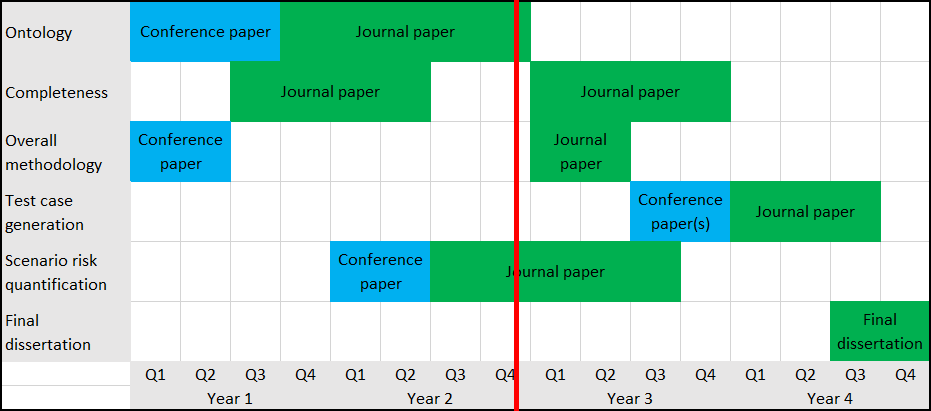
\includegraphics[width=\linewidth]{planning}
	\caption{Planning of my PhD. The red line denotes the time at writing this report.}
	\label{fig:planning}
\end{figure}

\section{Questions}

\begin{itemize}
	\item I think we discussed that previous time, but I am not sure. We planned our yearly progress meeting the 16th of October. Should I prepare some self-evaluation (one/two pages) for that meeting? Anything else that I need to prepare?
\end{itemize}


\printbibliography

%\clearpage
%\includepdf[pages=-,pagecommand={},width=\paperwidth]{../../""/.pdf}

\end{document}